\documentclass[a4paper, 11pt, final, garamond]{book}
\usepackage{cours-preambule}

\makeatletter
\renewcommand{\@chapapp}{Devoir surveill\'e -- num\'ero}
\makeatother

\begin{document}
\setcounter{chapter}{8}

\def\lspace{25}

\chapter{Commentaires sur le DS n\degree09}
\section{Commentaires généraux}

% \begin{figure}[htbp!]
% 	\centering
% 	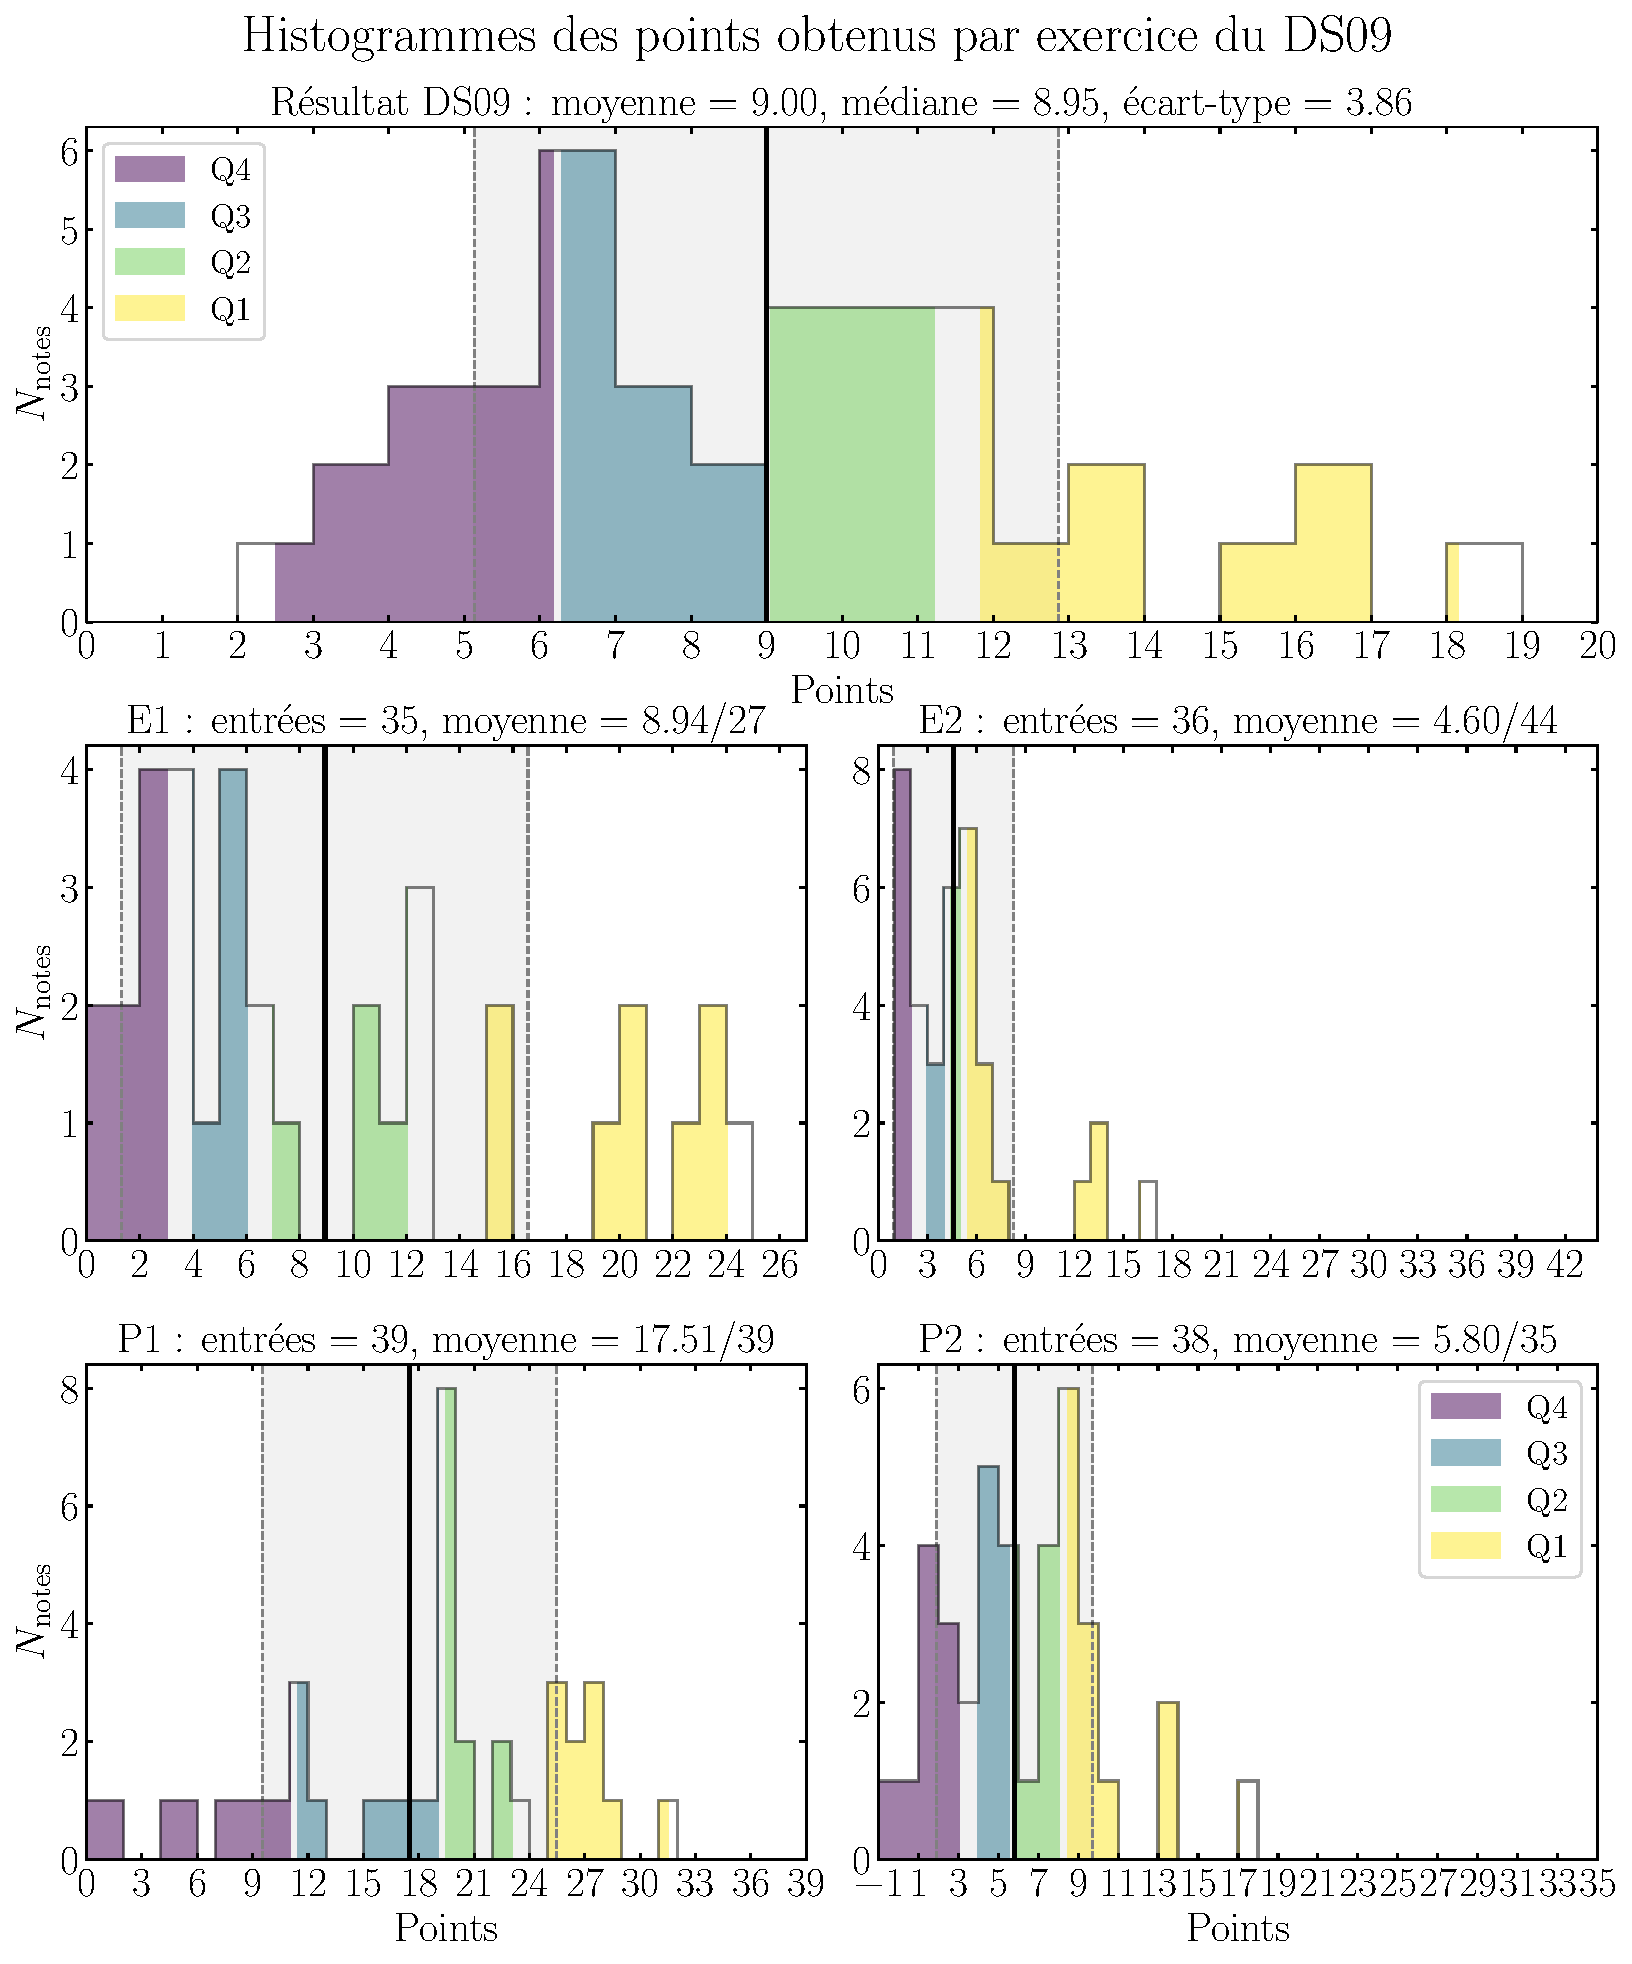
\includegraphics[width=1\linewidth]{DS09_hist_all}
% \end{figure}

\setcounter{section}{0}
\section[27]"E"{Étude de deux gaz parfaits dans un cylindre}
Exercice classique de début de thermodynamique, basé sur l'équilibre. N'inventez
pas des résultats (comme «~c'est isobare~»).
\bigbreak
\textbf{Attention}, dans ce genre d'énoncé de concours très commun
dans les petits concours, il faut justifier la réponse \textbf{sans raisonnement
	par l'absurde ou par élimination}. Vous devez \textbf{démontrer complètement} le
résultat.

\begin{enumerate}[label=\sqenumi]
	\item[n]{7} % Q1
	\item[n]{2} % Q2
	\item[n]{5} % Q3
	\item[n]{7} % Q4
	\item[n]{3} % Q5
	\item[n]{3} % Q6
\end{enumerate}

\section[43]"E"{Cycle de \textsc{Carnot}}
\begin{enumerate}[label=\sqenumi]
	\item[n]{3} % Q1
	Répondre à la partie sur le cycle.
	\item[n]{5} % Q2
	Bien.
	\item[n]{4} % Q3
	Ne partez pas dans des calculs à rallonge pour déterminer le rendement de
	\textsc{Carnot}~: c'est la démonstration en 3 lignes du cours en ayant
	$\frac{Q_C}{T_C} + \frac{Q_F}{T_F} = 0$, puisqu'alors $S\ind{cr} = 0$…
	\textbf{Bilan d'énergie $\equiv$ 1\ier{} ppe.}, et \textbf{bilan d'entropie
		$\equiv$ 2\up{d} ppe.}~!
	\item[n]{4} % Q4
	\item[n]{4} % Q5
	\item[n]{5} % Q6
	\item[n]{2} % Q7
	\item[n]{5} % Q8
	\item[n]{5} % Q9
	\item[n]{4} % Q10
	\item[n]{2} % Q11
\end{enumerate}

\setcounter{section}{0}
\section[39]"P"{Moteur de \textsc{Stirling}}
\begin{enumerate}[label=\sqenumi]
	\item[n]{6} % Q1
	\item[n]{4} % Q2
	\item[n]{8} % Q3
	\item[n]{3} % Q4
	\item[n]{3} % Q5
	\item[n]{2} % Q6
	\item[n]{3} % Q7
	\item[n]{5} % Q8
	\item[n]{3} % Q9
	\item[n]{2} % Q10
\end{enumerate}

\section[35]"P"{Étude thermodynamique d'une chambre froide}
\begin{enumerate}[label=\sqenumi]
	\item[n]{3} % Q1
	\item[n]{3} % Q2
	\item[n]{1} % Q3
	\item[n]{5} % Q4
	\item[n]{2} % Q5
	\item[n]{2} % Q6
	\item[n]{2} % Q7
	\item[n]{2} % Q8
	\item[n]{4} % Q9
	\item[n]{2} % Q10
	\item[n]{2} % Q11
	\item[n]{3} % Q12
	\item[n]{2} % Q13
	\item[n]{2} % Q14
\end{enumerate}

\end{document}
